\chapter{Discussion}
\label{chapter:discussion}
\section{Discussion}

\subsection{Power Supply}
\label{subsec:psdiscussion}
In this section a comparison is made between the simulated characteristics of the power supply and the measured results: where $D_{V_\text{Av}}$[\%], $D_{I_\text{res}}$[\%], and $D_{u_\text{ripple}}$[\%] correspond to the deviation between the simulated and measured results:
\begin{figure}[H]
    \centering
    \begin{minipage}{0.48\textwidth}
        \centering
        \captionsetup{justification=raggedright, labelfont=bf}
        \caption{Characteristics of the power supply in real-world applications under various load levels, using load resistors equipped with large heat sinks to dissipate the thermal energy from imperfect energy conversion. The data includes each load's average output voltage, current, and ripple percentage.}
        \begin{threeparttable}
          \centering
          
          \begin{tabular}{c @{\hspace{12pt}} *4{c} S @{\hspace{12pt}}}
            \toprule
            \multicolumn{5}{c}{\textbf{Deviation Power Supply Characteristic}} \\
            \cmidrule(lr){1-5}
            & & \multicolumn{3}{c}{\textbf{Deviations Performance Metr.}} \\
            \cmidrule(lr){3-5}
            & $R_\text{Load}$ [$\Omega$] & ${D_{V_\text{Av}}}$ [\%] & ${D_{I_\text{res}}}$ [\%] & ${D_{u_\text{ripple}}}$ [\%] \\
            \midrule
            1 & 19 & 9.84 & 10.08 & 25.19 \\
            2 & 38 & 7.65 & 8.53 & 16.08 \\
            3 & 76 & 6.83 & 7.41 & 41.03 \\
            4 & Open & 3.14 & - & -52.73 \\
            \bottomrule
          \end{tabular}
        \end{threeparttable}
        
        \label{tab:CharacteristicsSim}
    \end{minipage}\hfill
    \begin{minipage}{0.48\textwidth}
        \centering
        \resizebox{\linewidth}{!}{%
            \begin{tikzpicture} 
                \pgfplotsset{
                    every axis legend/.append style={at={(0.02,0.98)}, anchor=north west, legend columns = 1}, 
                    every axis/.append style={ytick distance=0.5, xtick distance=2, minor tick num=1, grid=major,
                    every axis grid/.append style={line width=0.5pt, draw opacity=0.4}}}
                \begin{axis} [xlabel = {Delivered power [W]}, ylabel = {Ripple [\%]}]
                 % First data set
                \addplot+[no markers, blue] table[row sep=crcr] 
                {
                    Supplied power(W):       Ripple(\%): \\  
                    21.31       3.23  \\
                    11.82     1.66  \\
                    6.351     1.10  \\
                    0     0.26  \\
                };
                \addlegendentry{Ripple [\%] - Measured}
                    \addplot+[no markers, red, dashed] table[row sep=crcr] {
                        Supplied Power (W):       Ripple(\%): \\  
                        17.63       2.58  \\
                        10.11     1.43  \\
                        5.54     0.78  \\
                        0     0.55  \\
                    };
                    \addlegendentry{Ripple [\%] - Simulated}
                \end{axis}
            \end{tikzpicture}%
        }
        \captionsetup{justification=raggedright, labelfont=bf}
        \caption{The output voltage ripple as a function of the power delivered to varying load resistances, showing the voltage ripple magnitude and the corresponding load power.}
        \label{fig:OutputVoltageRipplePower}
    \end{minipage}
\end{figure}

It can be seen that the difference between the simulated ripple voltage and the measured voltage is minimal. The same holds for the voltage and current values. This deviation can be caused by the physical characteristics of the smoothing capacitors and resistors. These components can have a deviation in their values, which can influence the output values. This does not cause great problems as all the requirements are still met. For future designs, it is therefore still recommended to use the same components.

As can be seen by comparing the simulation and measurement results in Fig. \ref{fig:OutputVoltageRipplePower}, it is clear that there is a significant discrepancy between them. This can be attributed to various factors:
\begin{itemize}
    \item The diodes used in the simulation differ from those used in reality. The 1N4148 diodes used in the simulation are general and are not fitted to carry large currents \cite{1n4148}. The 1N5408, on the contrary, can carry average rectified currents up to 3.0 A \cite{1n5408}. Therefore, the 1N5408 will result in much less loss over the diode.
    \item The transformer (CT-T) output voltage used in the simulation was set to 17${V_{\text{rms}}}$, whereas the measured output voltage was slightly higher at 17.25${V_\text{rms}}$. This small increase in voltage introduces a minor error in the simulated results, as the higher voltage directly affects the performance of the circuit.
    \item In the simulation, a 10mH inductor was used in series with the voltage source to simulate the transformer's impedance (CT-T's impedance). While this approach is reasonable, the real transformer's characteristics may slightly differ, leading to a small error and deviation in the results from the simulation when compared to the measurements.
\end{itemize}

As shown in Fig. \ref{fig:OutputCurrenteWith-Without}, the inclusion of smoothing capacitors results in a significant spike in the current, often referred to as rush-in current. This surge can be attributed to the charging process of the capacitors when they are first connected to the circuit. While the smoothing capacitors effectively reduce the ripple percentage and improve the stability of the output voltage $V_{\text{out}}$, this high initial current could potentially damage other components in the circuit if not properly managed.

This observation underscores the importance of carefully selecting the capacitor size to strike a balance between reducing ripple and minimizing the rush-in current. Exceeding an upper limit for the capacitor size could lead to reliability issues for the circuit components, emphasizing the need for circuit protection measures such as inrush current limiters (ICL) or thermistors (NTC, PTC) in future designs. 

\subsubsection{Future recommendations:}
Recoonmendations for improving the methodologies of the Power Supply subgroups include:
\begin{itemize}
    \item Implement the right components in the simulation since different diodes were used in the simulations compared to the actual design.
    \item Measure the output voltage of the transformer and implement this in the simulation.
    \item Measure the impedance of the transformer and implement this in the simulation.
\end{itemize}


\subsection{Power Amplifier}

\subsubsection{Analysis of Results}

The results obtained from the project show that the designed power amplifier closely aligns with the intended specifications. The pass-band gain of 24.83 is close to the desired gain of 25. Similarly, the measured cutoff frequencies of 20.9 Hz and 40.4 kHz almost meet requirement 1. The deviations observed in both gain and frequency response are insignificant and do not affect the amplifier's practical performance. Furthermore, the DC offset at the output of the function generator gets amplified by less than 1, which meets requirement 3 mentioned earlier for the power amplifier circuit.

To illustrate these deviations, the table below compares the ideal, simulated, and measured values, along with percentage deviations:
\begin{table}[H]
    \centering
    \captionsetup{justification=raggedright, labelfont=bf}
    \caption{Comparison of required, simulated, and measured values and deviations between the parameters for B2-1's power amplifier circuit. The deviation D$_{\text{diff},1}$ represents the difference between the simulated and required values, while D$_{\text{diff},2}$ corresponds to the difference between the measured and required values.}
    \resizebox{\textwidth}{!}{
    \begin{tabular}{c @{\hspace{12pt}} *7{c} S @{\hspace{12pt}}}
        \toprule
        \multicolumn{7}{c}{\textbf{Comparison Table for B2-1 Power Amplifier Performance}} \\
        \cmidrule(lr){1-7}
       
        & Parameter & Calculated Value & Simulated Value & Measured Value & D$_{\text{diff},1}$ [\%] & D$_{\text{diff},2}$ [\%]  \\
        \midrule
        Lower Cut-off & $f_\text{cut-off}$ [Hz] & 20.0Hz & 20.1Hz & 20.9Hz & 0.50\% &  4.50\% \\
         \vspace{10pt} \\
        Upper Cut-off & $f_\text{cut-off}$ [Hz] & 40.0kHz & 40.3kHz & 40.4kHz & 0.75\% & 1.00\% \\
         \vspace{10pt} \\
        Pass-band voltage gain &  $G_{\text{Gain}}$ & 25.0 & 24.60 & 24.83 & -1.60\% & -0.68\%  \\
        
        
        \bottomrule
    \end{tabular}
    }
\end{table}

The alternate power amplifier design was also assessed, achieving a gain of 26.6 with cut-off frequencies at 20Hz and 34kHz. The table below compares these values to those of the chosen amplifier and the specified requirements, including the percentage deviations:
\begin{table}[H]
    \centering
    \captionsetup{justification=raggedright, labelfont=bf}
    \caption{Comparison of required, simulated, and measured values and deviations between the parameters for B2-2's power amplifier circuit. The deviation D$_{\text{diff},1}$ represents the difference between the simulated and required values, while D$_{\text{diff},2}$ corresponds to the difference between the measured and required values.}
    \resizebox{\textwidth}{!}{
    \begin{tabular}{c @{\hspace{12pt}} *7{c} S @{\hspace{12pt}}}
        \toprule
        \multicolumn{7}{c}{\textbf{Comparison Table for B2-1 Power Amplifier Performance}} \\
        \cmidrule(lr){1-7}
       
        & Parameter & Calculated Value & Simulated Value & Measured Value & D$_{\text{diff},1}$ [\%] & D$_{\text{diff},2}$ [\%]  \\
        \midrule
        Lower Cut-off & $f_\text{cut-off}$ [Hz] & 20.0 Hz & 20.4 Hz & 19.5 Hz & 2.00\% & -2.56\% \\
         \vspace{10pt}\\
        Upper Cut-off & $f_\text{cut-off}$ [Hz] & 40.0 kHz & 40.0 kHz & 34.0 kHz & 0.00\% & -15.00\% \\
         \vspace{10pt}\\
        Pass-band voltage gain & $G_{\text{Gain}}$ & 25.0 & 24.90 & 26.60 & -0.40\% & -5.60\%  \\
        
        
        \bottomrule
    \end{tabular}
    }
\end{table}

The small deviations observed between the simulated and measured results in the above two tables can be attributed to several factors:
\begin{enumerate}
    \item \textbf{Component Tolerances:} Real-world resistors and capacitors exhibit variations of up to 20\% from their nominal values, affecting the frequency response and gain. These variations result in slight discrepancies between the measured and simulated results.
    \item \textbf{Non-Ideal Op-Amps:} The LM3886 op-amp exhibits non-ideal characteristics, including input offset voltage and a finite gain-bandwidth product, which cause discrepancies from ideal calculations.
    \item \textbf{Soldering and Connections:} Small resistances or imperfect connections during soldering may have slightly altered the circuit's behavior, leading to deviations from the expected performance.
\end{enumerate}

\subsubsection{Final Circuit Choice}
Will all the information gathered, it is now possible to select the power amplifier to be used in the final loudspeaker system. To make this decision, both systems are compared against the requirements outlined in Sec. \ref{requirements PA}:

 
\label{section: choosing a circuit}
\begin{itemize}[H]
    \item \textbf{Requirement 1:} The lower cut-off frequency of B2-1's amplifier is 20.9Hz, which is slightly father from the desired 20Hz compared to B2-2's amplifier, which achieved a cut-off frequency of 19.5Hz. However, the upper cut-off frequency of B2-1's amplifier is 40.4kHz, which is closer to the desired value than B2-2's cut-off of 34.4kHz.
    \item \textbf{Requirement 2:} The gain of B2-1's power amplifier ended up at 24.83, while B2-2's circuit reached a gain of 26.6. Therefore B2-1's power amplifier circuit is closer to the desired and required factor of 25 voltage gain and is less likely to cause speaker clipping at certain frequencies.
    \item\textbf{Requirement 3:} There was no significant difference between the two amplifier circuits in terms of the amount of DC offset eliminated.
\end{itemize}
After evaluating these three key requirements, the decision was made to use B2-1's power amplifier in the final system. Two out of the three requirements were much closer to the desired values in B2-1 compared to B2-2. The deviations in B2-1's power amplifier do not affect its ability to amplify the correct frequencies at the proper rate; These results demonstrate that the design approach was effective, and the chosen amplifier performs as expected, making it suitable for the required real-world applications.

\subsubsection{Phase}
The kink (abrupt change) observed in the phase response \autoref{fig:freq response with phase} remains unexplained. Despite thoroughly reviewing the derivations, no mistakes were found. Additionally, the discrepancy between the phase calculated using Python and the phase calculated by LTSpice is likely due to the different methods each tool uses to calculate the phase. While it is difficult to definitively determine which method yields a more accurate result, the Python-calculated phase has a higher likelihood of being close to the correct answer, as the phase should not reach values of 150 or -150 degrees at any point in the graph (see \autoref{fig:real circuit results}). However, since the measurements in \sfautoref{fig:freq response with phase} match the simulations closely, the phase shown in the same graph is likely to closely match the phase if it were measured.






\newpage
\subsection{Loudspeaker and Filters}
\subsubsection{Loudspeaker Models}
While the loudspeaker model aligns with the physical circuit's general shape and impedance frequency behavior, some discrepancies remain. The most notable is the reduced accuracy of the tweeter's model compared to the other speaker models. This could likely be because the model is better suited for speakers with lower resonant frequencies. Additionally, at frequencies below and above the resonance peak, the model tends to underestimate the total impedance $Z_{\text{tot}}$ of all three speakers, with the tweeter experiencing the greatest deviation.

However, the model performs very well in predicting the impedance behavior around the resonance peaks, which is the critical frequency range where the speaker operates most effectively. This accurate representation of the resonance frequencies ensures the model remains valuable for its primary purpose.

\subsubsection{Filters}
The design methodology was effectively implemented, enabling the filters to be built on time and allowing sufficient opportunity for evaluation. While there was room for improving efficiency through better communication between the three groups, the overall process was carried out in a well-structured manner.

Simulations conducted using LTSpice played a critical role in the filter development process, providing the group with a means to verify their design and refine their understanding. As shown in \sfautoref{fig:freq_resp}, the resulting frequency response is not entirely flat, exhibiting a maximum deviation of 5.0dB at approximately 510Hz. This deviation was deemed acceptable, as further adjustments to component values shifted the cut-off frequency into less favorable ranges, compromising the overall performance of the filter.

The insights gained from these simulations enabled thoughtful refinement of the filters. However, the reliance on simulations may have been excessive. While real-world testing was conducted, incorporating more frequent hands-on testing could have provided additional practical validation and potentially expedited optimization.

Measurements confirmed the effectiveness of the chosen methodology. As shown in \sfautoref{fig:electric_response}, the electric frequency response of the three combined possible filters aligns well with the corresponding simulations. The maximum observed deviation is approximately 5.2dB at around 1000Hz, which is acceptable since further tuning resulted in undesirable shifts in cut-off frequencies.

This behavior aligns with the simulations shown in \sfautoref{fig:freq_resp}, where a similar dip of approximately 4.5dB is observed near 100Hz. Analysis of the simulation indicates that this dip coincides with a phase shift from -180$^{\circ}$ to +180$^{\circ}$, causing signal deconstructive interference at this frequency. The differences between measurements and simulations are minor and can be attributed to the use of real components, which inherently deviate slightly from their ideal values, leading to small measurement discrepancies.

The chosen and the alternate filter responses were then compared. The acoustic response of both aggregated filters, measured at a distance of 1 meter, is shown in \sfautoref{fig:combined_response_with_alternate} 
\begin{figure}[H]
    \centering
    \begin{subfigure}[t]{0.48\textwidth}
        \centering
        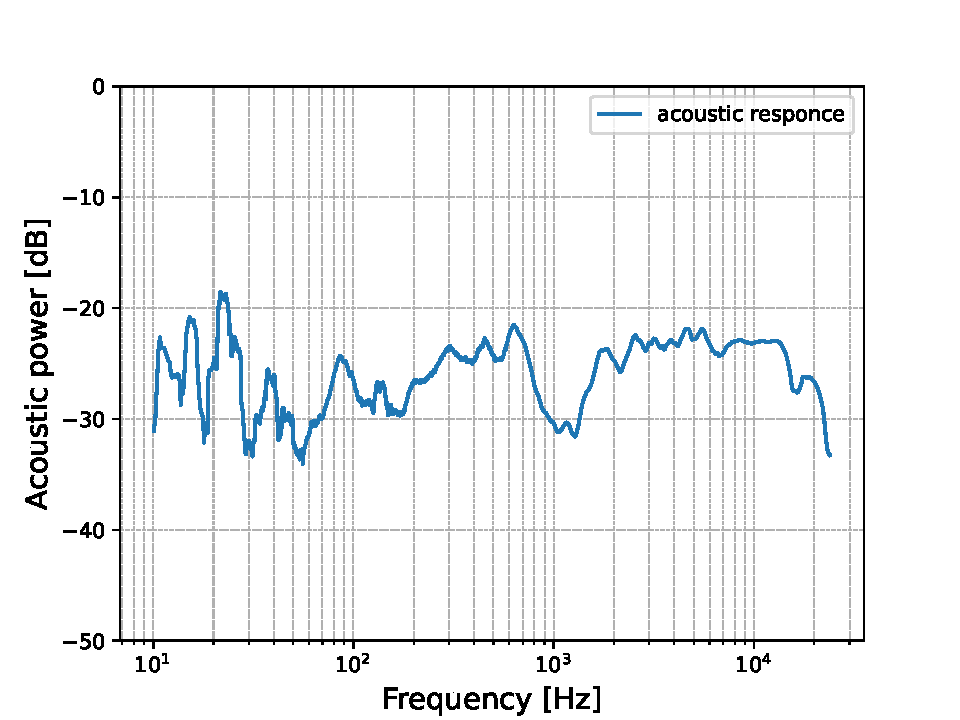
\includegraphics[width=\textwidth]{TU Delft Booming Bass Project Report/figures/FilterGroup/acoustic_response.pdf}
        \caption{The acoustic response of the chosen filter.}
        \label{fig:frequency_response}
    \end{subfigure}
    \hfill
     \begin{subfigure}[t]{0.48\textwidth}
         \centering
        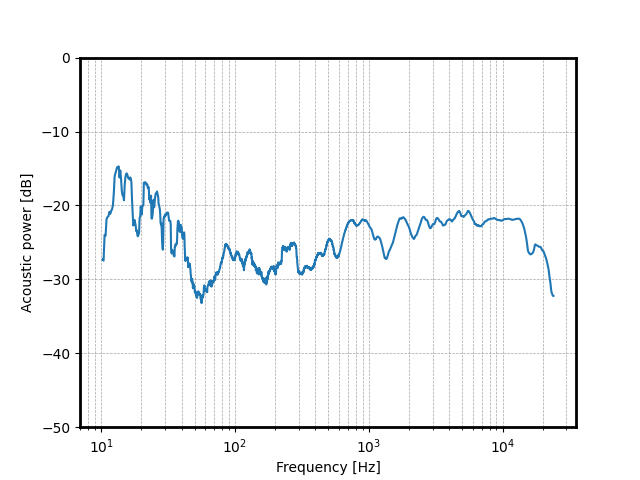
\includegraphics[width=\textwidth]{TU Delft Booming Bass Project Report/figures/FilterGroup/response_of_alternate_filterbank.png}
        \caption{The acoustic response of the alternate filter.}
        \label{fig:freq response alternate}
    \end{subfigure}
    
    \captionsetup{justification=raggedright, labelfont=bf}
    \caption{(L-R) Comparison between 2 filter banks: the chosen and alternate designs. The chosen filter exhibits a noticeably flatter acoustic response compared to the alternate filter.}
    \label{fig:combined_response_with_alternate}
\end{figure}

Both aggregated filters, each comprising their respective low-pass, band-pass, and high-pass filters, exhibit similar but slightly different acoustic power patterns. These differences primarily arise from variations in crossover frequencies and corresponding component values present in the filter circuits.

In the frequency range of 100Hz to 200Hz, the alternate filter demonstrates a higher maximum acoustic response compared to the chosen design. Additionally, the alternate design offers an advantage with a less pronounced dip in acoustic response between 1kHz and 2kHz. However, as the primary objective is to achieve the flattest frequency/acoustic response with the smallest maxima and largest minima, the response shown in \sfautoref{fig:frequency_response} for the chosen design remains the preferred option. 

\subsection{Future Recommendations}
The amplifier design process is long and involves many steps. It requires many parts to come together in an orderly fashion to create the amplifier successfully. While the three subgroups were able to create an amplifier that accurately recreated audio, adjustments to the methodology could have improved the design and construction of the components. 

For the design methodology, filter groups could have worked together more closely to find the component values for their filters. Currently, all three groups wrote different code and did their own Python simulations. By all using the same code, for example, they would have significantly reduced the time of the design process. Moreover, the filter groups could have done more tests in the real world of their filters, rather than relying on simulations in LT-Spice for adjusting the component values of the filters. It was highlighted that real-world tests gave the best insight into the quality of the filter. Therefore it would have been beneficial to the synthesis stage of the process.

Most of the steps taken in the design of the chosen power amplifier got quite accurate results. For that reason, the only future recommendation that could be made is to look again at the formula for the calculation of the phase in \ref{chapter:measurements}.  The derivation of this formula was gone over several times and a mistake was not found. So it would probably be beneficial to go over the transfer function again to see if somewhere along the line a mistake was made, or if perhaps the whole method of obtaining the function should be different by trying different ones. Furthermore a more accurate result for the phase shift could be obtained by measuring the phase at each frequency point chosen for measurements for this power amplifier.